\documentclass[10.5pt,a4paper]{article}
\usepackage[margin=2.1cm]{geometry}
\usepackage[T1]{fontenc}
\usepackage[utf8]{inputenc}
\usepackage{lmodern}
\usepackage{microtype}
\usepackage{booktabs}
\usepackage{graphicx}
\usepackage{longtable}
\usepackage{amsmath,amssymb}
\usepackage{xcolor}
\usepackage{caption}
\usepackage{subcaption}
\usepackage{enumitem}
\usepackage[colorlinks=true,linkcolor=blue!50!black,urlcolor=blue!50!black,citecolor=blue!50!black]{hyperref}
\setlist{itemsep=1pt,topsep=3pt}
\captionsetup{font=small,labelfont=bf}
\graphicspath{{../artifacts/plots/}}
\newcommand{\code}[1]{\texttt{\small #1}}
\makeatletter\newcommand{\inputtable}[1]{\@@input #1 }\makeatother

\title{\textbf{Predicting income above \$50K on the Adult census data}\\[2pt]
\large An end-to-end supervised-learning proof-of-concept\\[2pt]
\normalsize Applied ML: Foundations, Engineering \& Evaluation (MSA-DATI07-05) --- Albert School}
\author{Sofyan Hadj-Ali \and Martin Vallée \and Henry Falcon de Longevialle \and Kaled Goatache}
\date{November 2026}

\begin{document}
\maketitle
\vspace{-1em}
\begin{center}
\fbox{\parbox{0.92\textwidth}{\small
\textbf{Dataset used:} Option 1 --- Adult / Census Income, \code{fetch\_openml(name="adult", version=2)}.
Binary target: \code{class = ">50K"}. Sensitive attribute audited: \code{sex}.\\
\textbf{Code:} \url{https://github.com/Sofyan-Hdj/APML_project} \quad (\code{make all} reproduces every number and figure.)}}
\end{center}

\section{Problem framing and exploratory analysis}

\paragraph{Business framing.} We treat the task as a targeting problem: an institution (e.g.\ a bank
pre-qualifying people for a premium product) wants to flag individuals whose yearly income exceeds
\$50K from census-type attributes. Both errors cost something: a false positive wastes an offer and may
lead to an unaffordable product; a false negative is a missed customer. Because the positive class is
the minority and both errors matter, we use \textbf{PR-AUC} (average precision) as the threshold-free
selection metric, and \textbf{F1} at a tuned threshold, with precision, recall and balanced accuracy, as
operating-point metrics. Plain accuracy is reported only to show how misleading it is: always predicting
``$\le$50K'' already reaches 76.1\%.

\paragraph{Data.} 48{,}842 rows, 14 features (6 numeric, 8 categorical). We drop 52 exact duplicate
rows (features and label identical) so that the same individual cannot appear in both training and test,
leaving 48{,}790 rows. Key observations (Fig.~\ref{fig:eda}):
\begin{itemize}
  \item \textbf{Imbalance:} 23.9\% positives. Imbalanced but not extreme (ratio 1:3.2).
  \item \textbf{Missing values:} only in \code{workclass} (2{,}795), \code{occupation} (2{,}805) and
  \code{native-country} (856), 7.4\% of rows. Missing \code{workclass} and \code{occupation} occur
  together and concern mostly people outside the labour force: they are \emph{not missing at random} and
  their positive rate is far below average, so the missingness itself is informative.
  \item \textbf{Skewed capital variables:} \code{capital-gain} is 0 for 91.7\% of people and
  \code{capital-loss} for 95.3\%, with a long tail up to 99{,}999 (a top-coded value).
  \item \textbf{Redundancy:} \code{education} is a 1-to-1 label of the ordinal \code{education-num};
  \code{fnlwgt} is a census sampling weight (how many people the row represents), not an attribute of the
  person.
  \item \textbf{Sensitive attribute:} women are 33.2\% of the data but have a 10.9\% positive rate against
  30.4\% for men. \code{relationship} (\textit{Husband}/\textit{Wife}) is an almost perfect proxy for sex.
\end{itemize}

\begin{figure}[h]
\centering
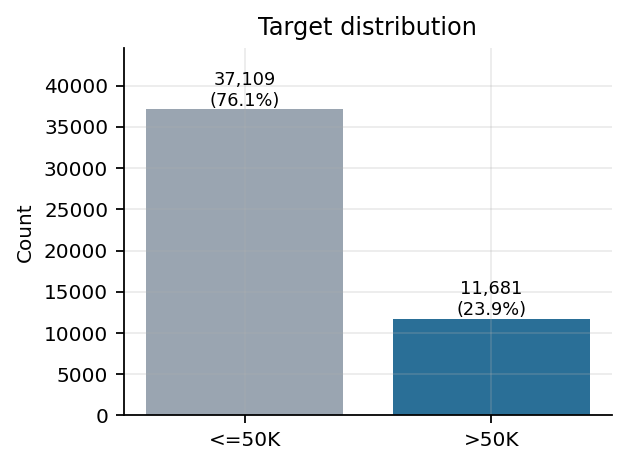
\includegraphics[width=0.24\textwidth]{eda_target.png}\hfill
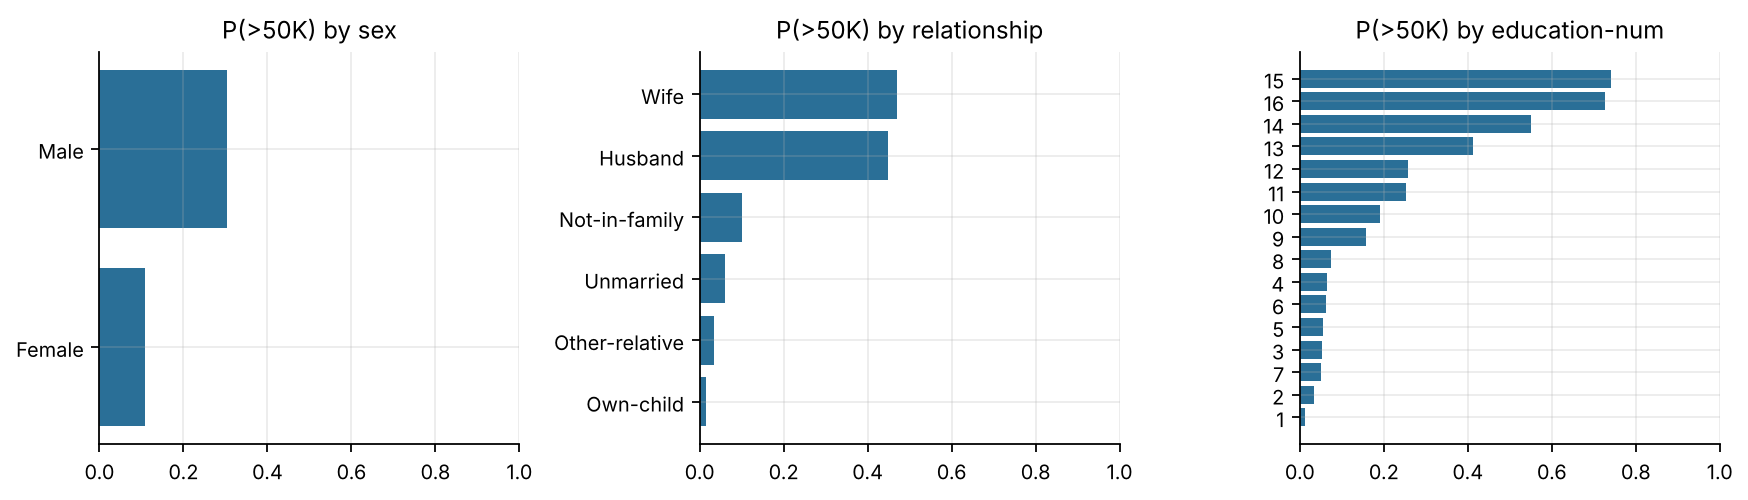
\includegraphics[width=0.74\textwidth]{eda_rate_by_group.png}
\caption{Class balance (left) and positive rate by sex, relationship and education level (right).}
\label{fig:eda}
\end{figure}

\paragraph{Honest train / validation / test split.} We use a stratified 60/20/20 split (seed 42):
\textbf{train} (29{,}274 rows) is the only data seen by hyper-parameter tuning, through 5-fold stratified
cross-validation; \textbf{validation} (9{,}758) is used for every post-training decision (model
selection, decision threshold, probability calibration, fairness post-processing); \textbf{test}
(9{,}758) is scored once at the end. All three splits keep the 23.9\% prevalence. All preprocessing is
inside the Pipeline (Section~\ref{sec:pipeline}), so imputation statistics, rare-category lists and
encoders are re-fitted on each CV training fold and never see held-out rows. We considered a time-based
split, but the 1994 census extract has no time dimension, so a random stratified split is appropriate.

\section{Feature engineering}
All engineering is done by a custom scikit-learn transformer, \code{FeatureEngineer}
(\code{src/adult\_poc/features.py}), followed by a \code{ColumnTransformer}.
\begin{itemize}
  \item \textbf{\code{capital\_net\_log}} $=\operatorname{sign}(g-\ell)\log(1+|g-\ell|)$ with $g$, $\ell$ the
  capital gain and loss. The raw columns are 90\%+ zeros with extreme tails; the signed log of the net
  amount compresses the tail (helping the linear model) while keeping the direction. It turns out to be the
  most important feature (Section~\ref{sec:shap}).
  \item \textbf{\code{has\_capital\_gain}, \code{has\_capital\_loss}}: owning investments at all is a wealth
  signal, independently of the amount declared that year.
  \item \textbf{\code{is\_married}}: collapses the 7 \code{marital-status} levels into the split that
  matters economically: living with a spouse (\textit{Married-civ-spouse}, \textit{Married-AF-spouse}), which
  goes with pooled household income and is the strongest single split in the EDA.
  \item \textbf{\code{overtime}} (more than 40\,h/week) and \textbf{\code{age\_sq}}: income rises with age then
  flattens and falls after about 55; the squared term lets the logistic regression model this inverted U.
  \item \textbf{Rare categories:} countries with fewer than 50 training rows are grouped into \textit{Other};
  the one-hot encoder also groups levels with fewer than 20 rows (\code{min\_frequency=20},
  \code{handle\_unknown="infrequent\_if\_exist"}), so an unseen category at serving time does not crash the API.
  \item \textbf{Dropped:} \code{fnlwgt} and \code{education} (see Section 1); raw capital columns are
  replaced by the engineered ones.
  \item \textbf{Missing values:} categorical NaNs become an explicit \textit{Missing} level (justified by the
  not-at-random pattern above); numeric columns (none missing here, but possible at serving time) use the
  training median. Numeric features are standardised for the logistic regression only.
\end{itemize}
After encoding, the models see 72 columns. A unit test (\code{tests/test\_pipeline.py}) checks the
engineered values on hand-made rows.

\section{Class imbalance}
\label{sec:imbalance}
\paragraph{Metrics.} At 24\% prevalence, accuracy and ROC-AUC look flattering even for weak models. We
therefore select on PR-AUC, whose baseline equals the prevalence (0.239), and report F1, precision,
recall and balanced accuracy at an explicit threshold.

\paragraph{Remedies compared.} \code{scripts/imbalance\_ablation.py} compares, on the validation set and
with default hyper-parameters, (i) no correction, (ii) cost-sensitive learning with
\code{class\_weight="balanced"} (each positive weighs $n/(2n_{+})\approx 2.1$, each negative $\approx 0.66$),
(iii) SMOTE and (iv) random under-sampling (both inserted in an \code{imblearn} Pipeline \emph{after}
preprocessing, so synthetic rows are built from training rows only), each with the default 0.5 threshold,
plus (i) and (ii) with an F1-optimal threshold chosen on validation (``+thr'').

\begin{table}[h]
\centering\small
\begin{tabular}{llcccccccc}
\toprule
Model & Remedy & PR-AUC & F1 & Prec. & Recall & Bal.\ acc. & Acc. & Brier & Thr. \\
\midrule
\inputtable{tables/imbalance_ablation.tex}
\bottomrule
\end{tabular}
\caption{Imbalance remedies on the validation set (default hyper-parameters).}
\label{tab:imb}
\end{table}

\paragraph{Findings and choice.} Table~\ref{tab:imb} shows that (1) no remedy changes the \emph{ranking}
quality much (PR-AUC within $\pm$0.006): resampling or reweighting does not create information; (2) with the
default 0.5 threshold, the uncorrected models are too conservative (LightGBM recall 0.665) and every remedy
moves the operating point towards recall; (3) once the threshold is tuned, the uncorrected and the weighted
models reach the same F1 (0.728 for LightGBM); (4) SMOTE and under-sampling bring nothing over weighting and
add a dependency and, for under-sampling, discard about 69\% of the negatives.

We kept \textbf{cost-sensitive learning (\code{class\_weight="balanced"}) combined with a validation-tuned
decision threshold} for all three models. It is the simplest remedy that works the same way across the
three model families (\code{models.py}: \code{build\_model} passes \code{class\_weight="balanced"} to
\code{LogisticRegression}, \code{RandomForestClassifier} and \code{LGBMClassifier}), and threshold tuning
(\code{metrics.best\_f1\_threshold}) sets the final operating point. The ablation also shows its cost:
reweighting raises the Brier score (0.088\,$\rightarrow$\,0.110 for LightGBM) because the scores are pushed
up. We keep this in mind and diagnose and correct it in Section~\ref{sec:calib}. A fair criticism is that
``no weighting + threshold'' would give the same F1 with better-calibrated raw scores; we discuss this in
Section~\ref{sec:conclusion}.

\section{Pipeline, models and tuning}
\label{sec:pipeline}
\paragraph{Single Pipeline.} Every model is wrapped as
\code{Pipeline([("features", FeatureEngineer()), ("preprocess", ColumnTransformer(...)), ("model", clf)])}
(\code{features.make\_pipeline}). The fitted object takes the raw census DataFrame and returns
probabilities. It is what we cross-validate, save with \code{joblib}, explain, calibrate and serve.

\paragraph{Model progression.} (1) \textbf{Logistic regression} with elastic-net penalty (\code{saga}),
a transparent baseline; (2) \textbf{Random Forest}, which adds non-linearities and interactions with
low variance through bagging; (3) \textbf{LightGBM} gradient boosting, which reduces bias sequentially
and usually leads on tabular data.

\paragraph{Optuna with honest CV.} Each model is tuned with Optuna's TPE sampler (seeded) on the
\emph{training split only}. The objective of a trial is the mean PR-AUC over a 5-fold
\code{StratifiedKFold}; the whole Pipeline is refit inside every fold (\code{cross\_validate}), so
preprocessing never leaks. Validation and test data play no role in hyper-parameter choice, so the CV
score is not contaminated by validation or test data, but it is still slightly optimistic, since we keep the
best of 30 to 40 trials per model. The validation scores are the independent check (Table~\ref{tab:models}). Budgets: 30 trials for logistic regression ($C\in[10^{-3},10]$
log-scale, $\ell_1$-ratio $\in[0,1]$), 30 for Random Forest (number of trees, depth, leaf size,
\code{max\_features}, bootstrap fraction) and 40 for LightGBM (trees, learning rate, leaves, child samples,
row/column subsampling, $\ell_2$). Fig.~\ref{fig:optuna} shows the optimisation histories.

\begin{figure}[h]
\centering
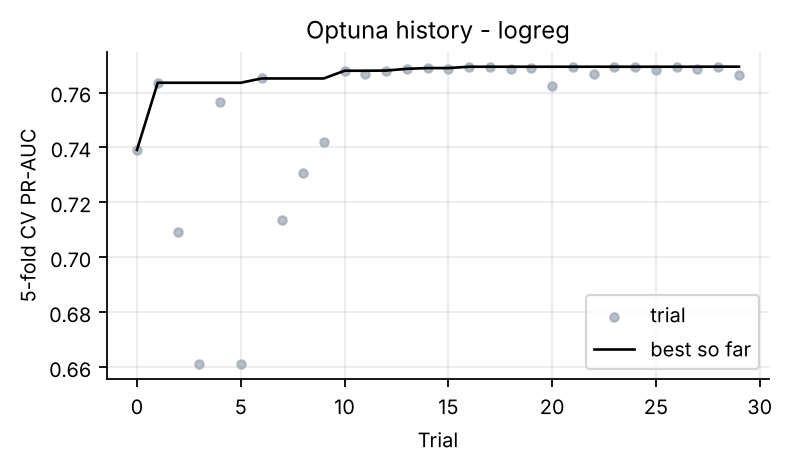
\includegraphics[width=0.32\textwidth]{optuna_history_logreg.png}\hfill
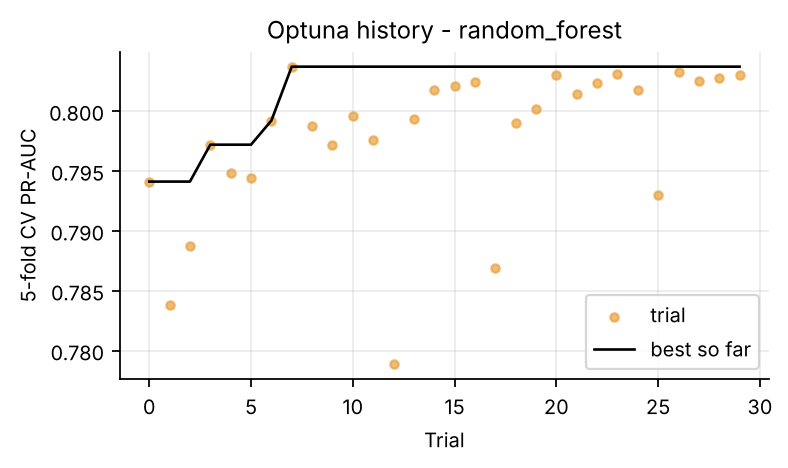
\includegraphics[width=0.32\textwidth]{optuna_history_random_forest.png}\hfill
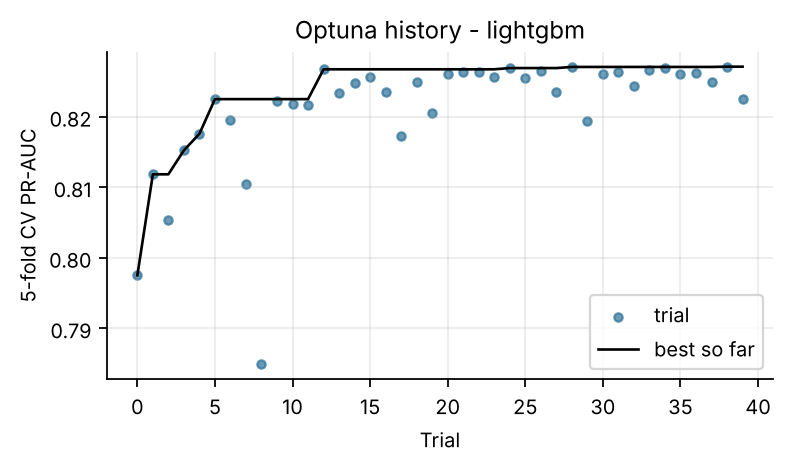
\includegraphics[width=0.32\textwidth]{optuna_history_lightgbm.png}
\caption{Optuna histories (5-fold CV PR-AUC per trial and running best). The logistic regression search is still improving near its last
trials (best at trial 28 of 30), so it has not converged; the random forest reaches its best at trial 7 and does not improve after it; LightGBM keeps improving until trial 38 of 40.}
\label{fig:optuna}
\end{figure}

Best configurations (all trials are in the run log, Appendix~\ref{app:runlog}):
\begin{itemize}
  \item Logistic regression (trial 28): $C=9.45$, $\ell_1$-ratio $=0.997$, i.e.\ almost pure lasso with weak
  regularisation: with 29k rows and 72 columns, the model is not variance-limited. CV PR-AUC
  $0.769\pm0.005$.
  \item Random Forest (trial 7): 350 trees, depth 13, min.\ leaf 2, 51\% of features per split, 66\% bootstrap.
  CV PR-AUC $0.804\pm0.004$.
  \item LightGBM (trial 38): 750 trees, learning rate 0.035, 16 leaves, min.\ child samples 18, 45\% of
  columns per tree, $\lambda_2=0.18$: many small trees with strong column subsampling.
  CV PR-AUC $0.827\pm0.005$.
\end{itemize}

\paragraph{Comparison.} Each tuned pipeline is refit on the full training split; its decision threshold is
the F1-optimal one on validation; the final model is chosen on validation PR-AUC. Test numbers are given for
completeness and were not used for any choice.

\begin{table}[h]
\centering\small
\begin{tabular}{llcccccccc}
\toprule
Model & Split & PR-AUC & ROC-AUC & F1 & Prec. & Recall & Bal.\ acc. & Brier & Thr. \\
\midrule
\inputtable{tables/model_comparison.tex}
\bottomrule
\end{tabular}
\caption{Same metrics for the three models: 5-fold CV mean on train (at threshold 0.5), validation and test
(at the validation-tuned threshold). The dummy classifier predicts the prior.}
\label{tab:models}
\end{table}

\begin{figure}[h]
\centering
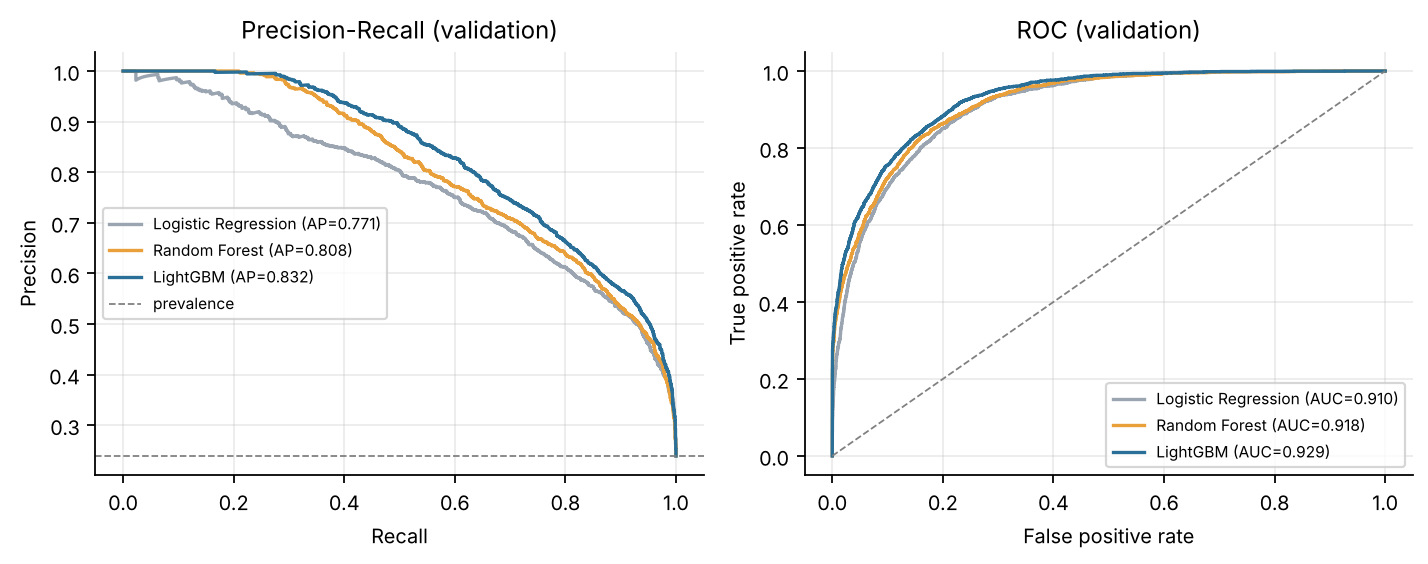
\includegraphics[width=0.85\textwidth]{model_pr_roc_val.png}
\caption{Precision--recall and ROC curves on the validation set. The PR view separates the models much more
clearly than ROC.}
\label{fig:prroc}
\end{figure}

\paragraph{What each step bought us.} Going from logistic regression to Random Forest adds
$+0.037$ validation PR-AUC and $+0.015$ validation F1: trees capture interactions the linear model cannot (e.g.\ the
return on education is much larger for married people) and thresholds on capital amounts. LightGBM adds
another $+0.024$ validation PR-AUC and $+0.019$ validation F1 and, at the chosen threshold, gets the best \emph{precision} (0.71
vs 0.64 for the forest) at a lower recall (0.75 vs 0.80): boosting fits the residual structure the forest averages
away. ROC-AUC gains are smaller (0.910\,$\rightarrow$\,0.918\,$\rightarrow$\,0.929), which shows why we use PR-AUC
for selection. The costs go the other way: the linear model is readable from its coefficients, while the
ensembles need SHAP (Section~\ref{sec:shap}); tuning time was 16\,min for the logistic regression
(\code{saga} converges slowly at high $C$), 12\,min for the forest and 5\,min for LightGBM on a 2-core
machine. Validation scores agree with the CV means within about one CV standard deviation
(Table~\ref{tab:models}), so the tuning did not overfit the folds. The test scores are higher than validation
for all three models, by 0.005 to 0.009 PR-AUC, and for the random forest and LightGBM they sit 2.6 to 2.8 CV
standard deviations above the CV mean. Because the shift is shared by all three models, it is more likely a
property of the test split than of any one model's tuning.

\textbf{Final model: LightGBM}, threshold 0.670. On the untouched test set: PR-AUC 0.840, ROC-AUC 0.933,
F1 0.735, precision 0.709, recall 0.763, balanced accuracy 0.832 (accuracy 0.868, against 0.761 for the
dummy). The threshold above 0.5 is what we expect: class weighting inflates the scores, and the validation
search moves the threshold back up.

\section{Explainability with SHAP}
\label{sec:shap}
We use \code{shap.TreeExplainer} on the LightGBM step of the fitted pipeline, applied to 2{,}000 test rows
transformed by the pipeline's preprocessing (\code{scripts/explain.py}). SHAP values are additive in
log-odds. To read importance at the level of business concepts, we also sum the mean $|$SHAP$|$ of the one-hot
columns of each original variable.

\begin{figure}[h]
\centering
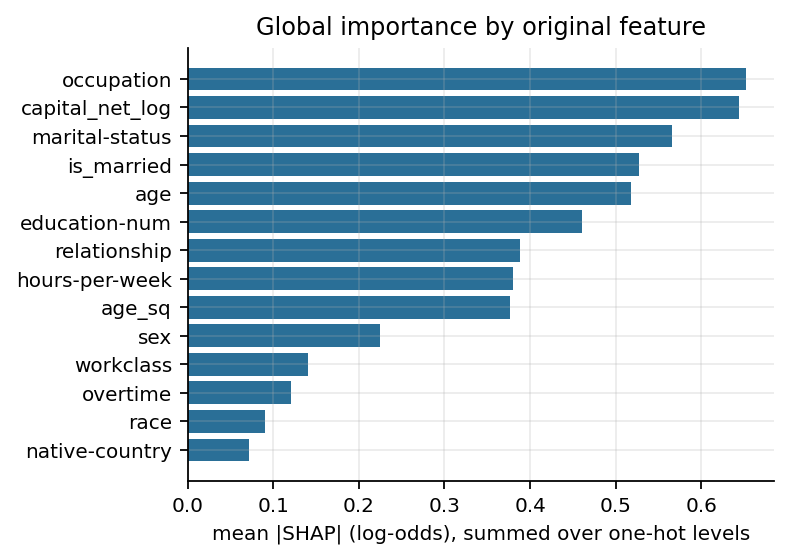
\includegraphics[width=0.40\textwidth]{shap_global_grouped.png}\hfill
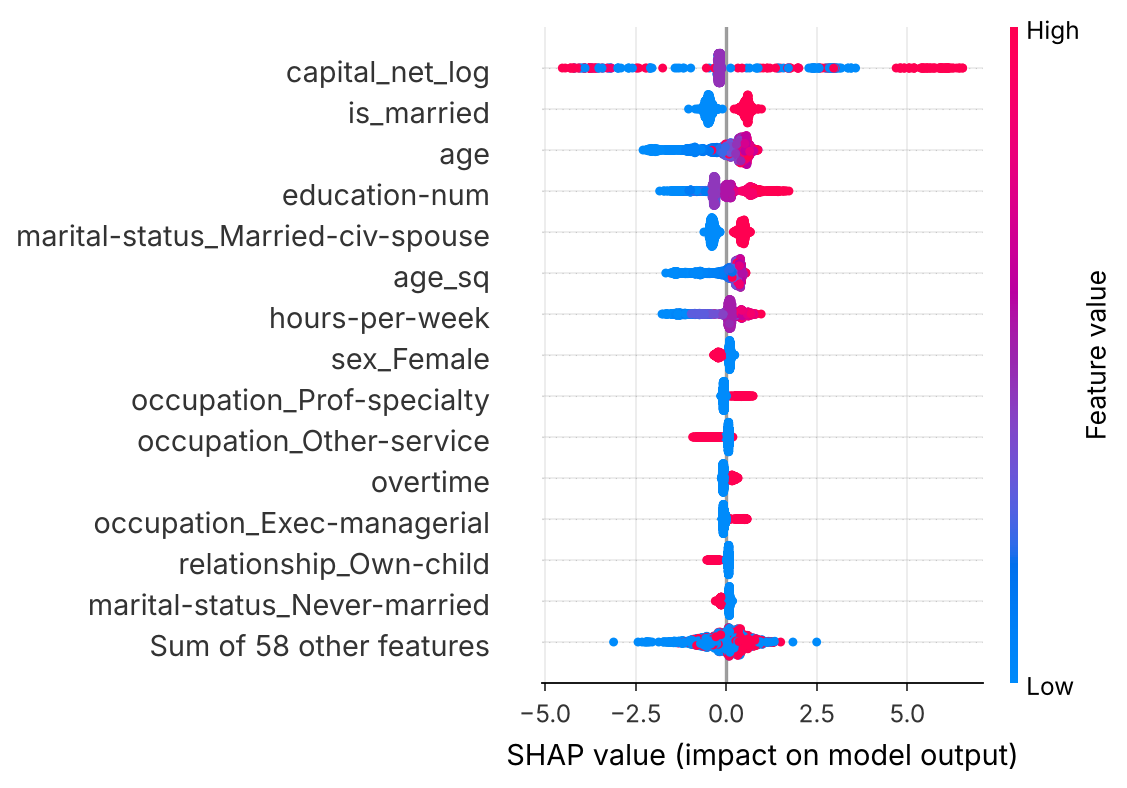
\includegraphics[width=0.57\textwidth]{shap_beeswarm.png}
\caption{Global importance. Left: mean $|$SHAP$|$ grouped by original feature. Right: beeswarm of the 15
most important encoded columns (colour = feature value).}
\label{fig:shapglobal}
\end{figure}

\paragraph{Global view.} The top drivers (Fig.~\ref{fig:shapglobal}) are \code{capital\_net\_log} (0.65),
\code{occupation} (0.64), marital status (\code{marital-status} 0.55 plus \code{is\_married} 0.52; the
model splits this signal between the two encodings), \code{age} (0.51, plus 0.37 for \code{age\_sq}),
\code{education-num} (0.45), \code{relationship} (0.37) and \code{hours-per-week} (0.37). \code{sex}
comes next (0.22), ahead of \code{workclass}, \code{race} (0.09) and \code{native-country} (0.07).

\paragraph{Do they make business sense?} Mostly yes. Investment income, a managerial or professional
occupation, education, experience (age, with diminishing returns visible in the beeswarm) and hours worked
are the textbook determinants of earnings. Marriage is less obvious: it is partly a life-cycle proxy
(older, more established people), and partly a consequence of how the census records income in a
\emph{household} context. Two points need care. (i) Large \emph{negative} \code{capital\_net\_log} values
(capital losses of about \$1{,}900--2{,}400) push predictions \emph{up}: declaring a capital loss requires
owning investments and, in US tax rules, is mostly worth doing for higher earners. This is a real pattern
but a fragile one: it depends on the tax rules of the time. (ii) \code{sex} has a direct effect
(\textit{Female} lowers the log-odds) on top of its proxies (\textit{Husband}/\textit{Wife}). The model
reproduces the historical pay gap in the data. It is ``accurate'', but it motivates the audit in
Section~\ref{sec:fair}.

\paragraph{Local explanations.} We explain five representative test predictions
(Fig.~\ref{fig:shaplocal}; the five waterfall plots are in \code{artifacts/plots/}):
\begin{itemize}
  \item \textbf{Confident true positive} ($p\approx1.00$): 41-year-old married executive with a doctorate and
  a \$15{,}024 capital gain; the capital gain alone adds $+5.95$ log-odds.
  \item \textbf{Confident true negative} ($p\approx0.00$): 17-year-old working 12\,h/week; age ($-2.0$),
  $age^2$ ($-1.4$) and short hours ($-1.3$) dominate.
  \item \textbf{False positive} ($p=0.99$, true $\le$50K): 51-year-old married male executive with a
  \$1{,}902 capital loss. The capital-loss pattern ($+2.4$), marriage and seniority all point up; the profile
  is typical of high earners, so the error is understandable and shows the limit of the capital-loss signal.
  \item \textbf{False negative} ($p=0.04$, true $>$50K): 56-year-old divorced woman in craft/repair with low
  formal education (\code{education-num}=5). Every typical signal points down; such ``atypical'' high earners
  are the ones a model based on correlations misses.
  \item \textbf{Borderline} ($p=0.67\approx$ threshold): 34-year-old married salesman, 50\,h/week, high-school
  level: marriage and long hours ($+0.55$, $+0.47$) are balanced by education ($-0.38$).
\end{itemize}

\begin{figure}[h]
\centering
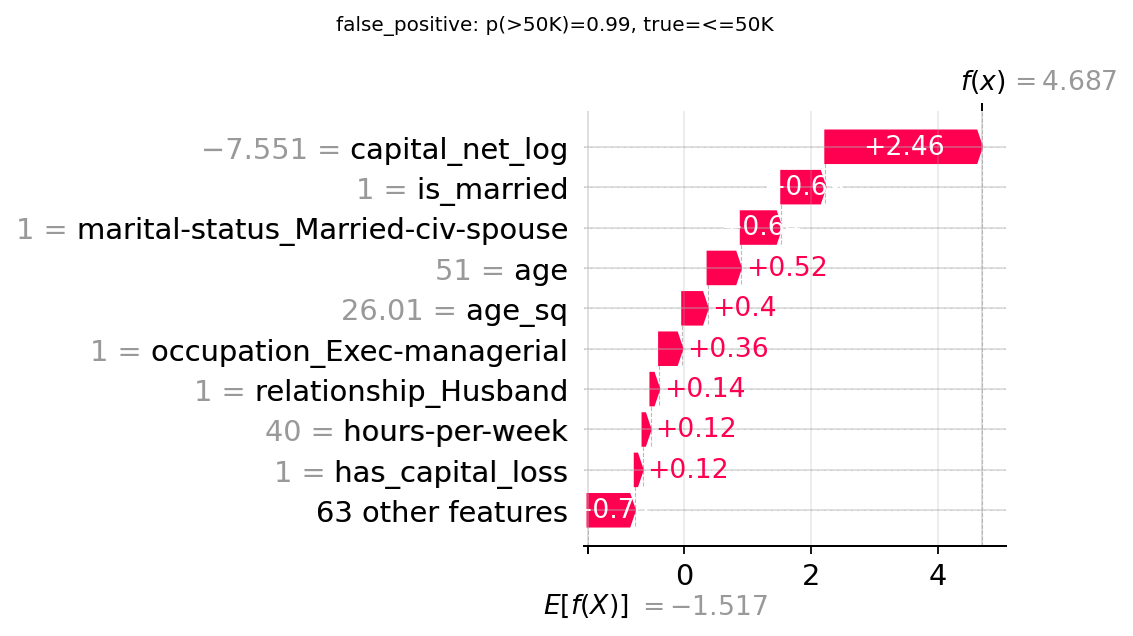
\includegraphics[width=0.49\textwidth]{shap_local_false_positive.png}\hfill
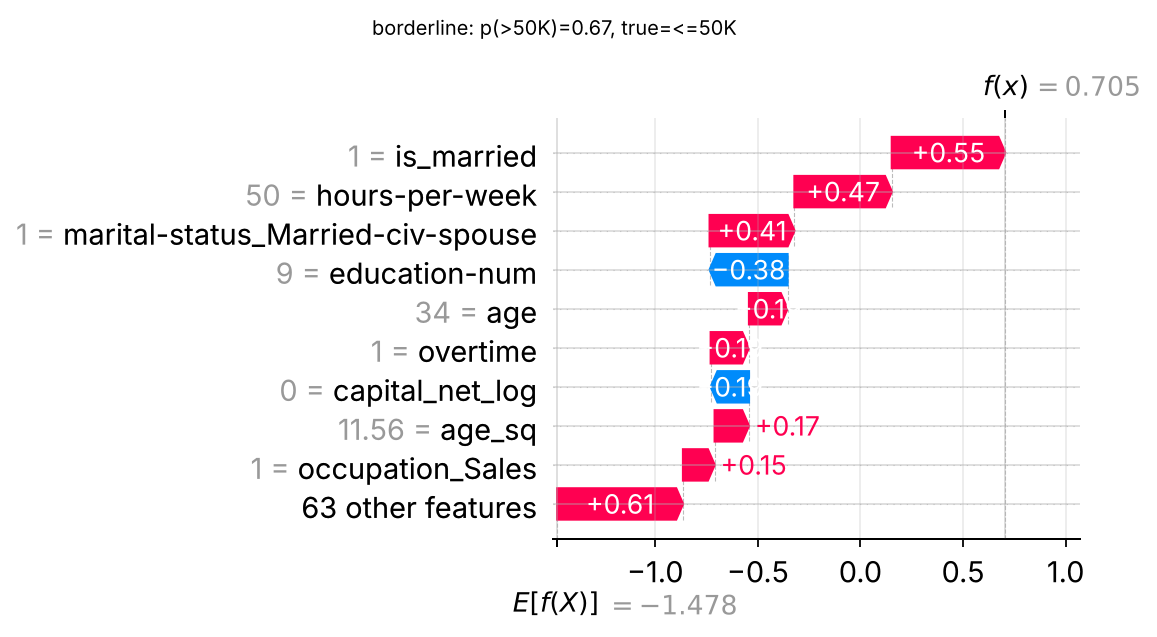
\includegraphics[width=0.49\textwidth]{shap_local_borderline.png}
\caption{SHAP waterfalls for the false positive (left) and the borderline case (right).}
\label{fig:shaplocal}
\end{figure}

\section{Calibration diagnostics}
\label{sec:calib}
\begin{figure}[h]
\centering
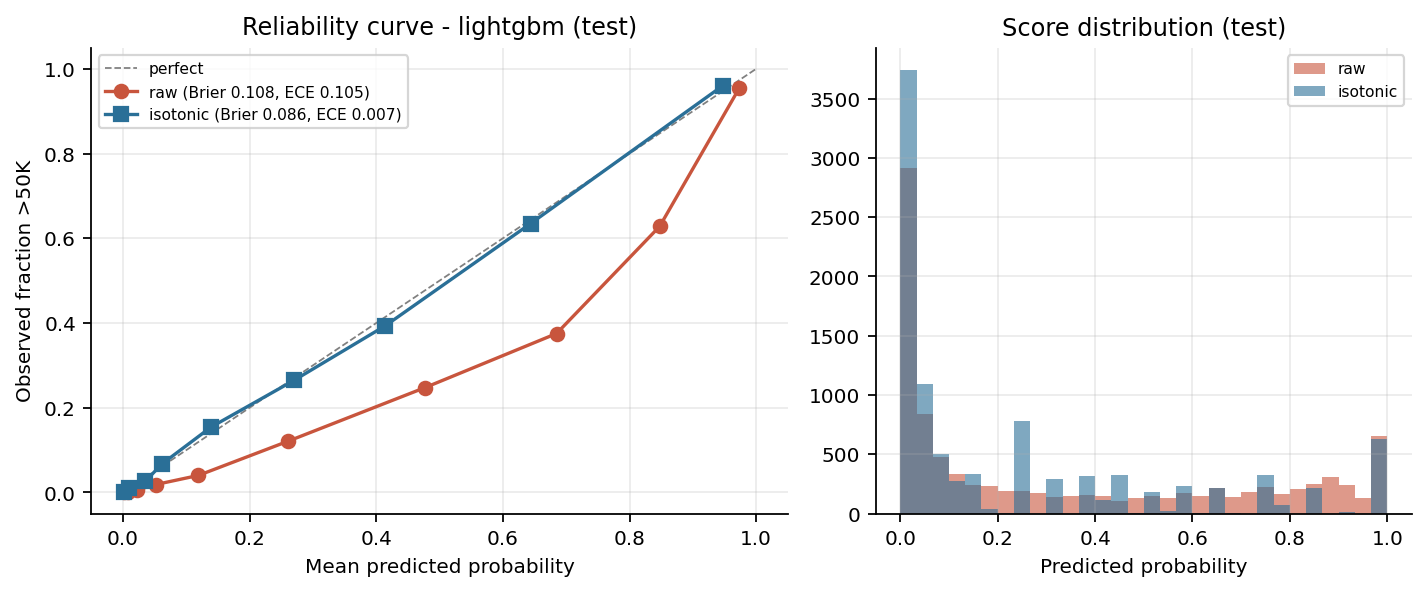
\includegraphics[width=0.85\textwidth]{calibration_reliability.png}
\caption{Reliability curve on the test set (10 quantile bins) for the raw LightGBM scores and after isotonic
recalibration fitted on the validation set; right: score distributions.}
\label{fig:calib}
\end{figure}

\paragraph{Diagnosis.} On the test set the raw LightGBM scores have a Brier score of \textbf{0.108} and an
ECE (10 equal-width bins) of \textbf{0.106}. The reliability curve (Fig.~\ref{fig:calib}) lies entirely
\emph{below} the diagonal: when the model says 0.48 the observed rate is 0.25; for 0.68 it is 0.37; for 0.85 it
is 0.63. The average predicted probability is 0.345 for an observed prevalence of 0.239. The model is
therefore \textbf{over-confident in the positive class}: it systematically over-estimates the probability
of earning more than \$50K. This is the expected side effect of \code{class\_weight="balanced"}: weighting
positives $\approx3.2\times$ relative to negatives shifts the learned log-odds by roughly $\log 3.2\approx1.2$.
Ranking is unaffected, which is why PR-AUC and the tuned-threshold decisions are fine.

\paragraph{Correction.} We fit an isotonic mapping on the \emph{validation} scores, keeping the trained
pipeline frozen (\code{CalibratedClassifierCV(FrozenEstimator(pipe), method="isotonic")}), and evaluate on
test: Brier drops to \textbf{0.085} (below the 0.088 of the unweighted model in Table~\ref{tab:imb}), ECE to
\textbf{0.006}, and the mean predicted probability becomes 0.240. Decisions are unchanged (same F1 0.735 at
the re-tuned threshold 0.41, the monotone image of 0.67). PR-AUC falls slightly (0.840\,$\rightarrow$\,0.828)
because isotonic regression is a step function that creates ties among scores. Platt scaling would avoid
this but assumes a sigmoid-shaped distortion.

\paragraph{Would we trust the probabilities?} \textbf{Not the raw ones.} They are fine for ranking and for the
tuned yes/no decision, but any downstream use that reads them \emph{as probabilities} (expected value of an
offer, a risk score shown to a human, a mix with other probabilities) would overstate the chance of high
income by about 10 points on average and up to 30 points in the middle bins. \textbf{After isotonic
recalibration we would} use them, with two caveats: the calibrator was fitted on 9.7k validation rows, so the
sparse upper bins are noisy; and calibration must be monitored if the population drifts. The API therefore
returns both the raw score and the calibrated probability.

\section{Fairness and bias audit}
\label{sec:fair}
\paragraph{Setting and definitions.} The sensitive attribute is \code{sex} (A $\in$ \{Female, Male\}). In our
targeting scenario, a positive prediction gives access to an offer, so we report: \textbf{demographic parity}
(equal selection rates $P(\hat Y=1\mid A)$); \textbf{equal opportunity} (equal true positive rates: people who
\emph{really} earn $>$50K should be found equally often regardless of sex); \textbf{equalized odds} (equal TPR
\emph{and} FPR; we report the larger of the two gaps); and \textbf{predictive parity} (equal precision). We
consider \textbf{equalized odds} the most relevant: it conditions on the true outcome, so it does not
require equal selection rates when base rates truly differ (11.5\% vs 30.4\% in the test set), but it does
require that errors are not distributed unequally between women and men. Demographic parity is reported
because the base-rate gap itself reflects historical discrimination, and a regulator may look at it.

\begin{table}[h]
\centering\small
\begin{tabular}{lccc}
\toprule
Metric (test set) & Baseline & Unawareness & ThresholdOpt (EO) \\
\midrule
\inputtable{tables/fairness_summary.tex}
\bottomrule
\end{tabular}
\hfill
\caption{Performance and fairness gaps on the untouched test set. ``Unawareness'': same LightGBM retrained
with \code{sex} removed from the inputs.}
\label{tab:fair}
\end{table}

\begin{table}[h]
\centering\small
\begin{tabular}{llccccc}
\toprule
Variant & Group & Selection rate & TPR & FPR & Precision & F1 \\
\midrule
\inputtable{tables/fairness_by_group.tex}
\bottomrule
\end{tabular}
\caption{Per-group metrics on the test set.}
\label{tab:fairgroup}
\end{table}

\paragraph{Audit of the final model.} At its single global threshold, LightGBM selects 9.5\% of women and
34.2\% of men (DP difference 0.247, ratio 0.28, far below the ``four-fifths'' rule of 0.8). Part of this
reflects the different base rates, but the error rates are unequal too: the TPR is 0.632 for women against
0.789 for men (\textbf{equal-opportunity gap 0.157}): a woman who really earns more than \$50K is missed
37\% of the time, against 21\% for a man. The FPR gap is 0.122 (0.025 vs 0.147). Precision is similar (0.77 vs
0.70). The race audit (secondary, not mitigated) shows comparable gaps (EO difference 0.173 between groups,
smaller groups being noisy).

\paragraph{Unawareness is not enough.} Retraining without \code{sex} barely changes anything (EO 0.147, DP
0.247): \code{relationship}, \code{marital-status}, occupation and hours carry the same information. This is
the classic proxy problem and the reason we keep \code{sex} available for auditing.

\paragraph{Mitigation: post-processing with \code{ThresholdOptimizer}.} We apply fairlearn's
\code{ThresholdOptimizer} with an \textbf{equalized-odds} constraint (objective: balanced accuracy) on top of
the frozen final pipeline. It learns group-specific (randomised) thresholds on the \emph{validation} set;
the test set stays untouched for the comparison. Results (Tables~\ref{tab:fair}--\ref{tab:fairgroup},
Fig.~\ref{fig:fair}):
\begin{itemize}
  \item The equalized-odds gap drops from 0.157 to \textbf{0.037} (TPR 0.830 vs 0.852; FPR 0.175 vs 0.212) and
  the DP gap from 0.247 to 0.156 (ratio 0.28\,$\rightarrow$\,0.62).
  \item The cost: F1 drops from 0.735 to 0.686 and accuracy from 0.868 to 0.814; balanced accuracy only from
  0.832 to 0.826. To equalise error rates, the optimiser \emph{raises} the women's TPR, which needs a much lower
  threshold for them, so their FPR rises from 0.025 to 0.175.
  \item \textbf{Precision parity gets worse} (gap 0.068\,$\rightarrow$\,0.254: precision for women falls to
  0.38). This is the impossibility result in practice: with different base rates, equalized odds and
  predictive parity cannot hold together. Choosing equalized odds is a value judgement that has to be made
  explicitly with the business owner.
\end{itemize}

\begin{figure}[h]
\centering
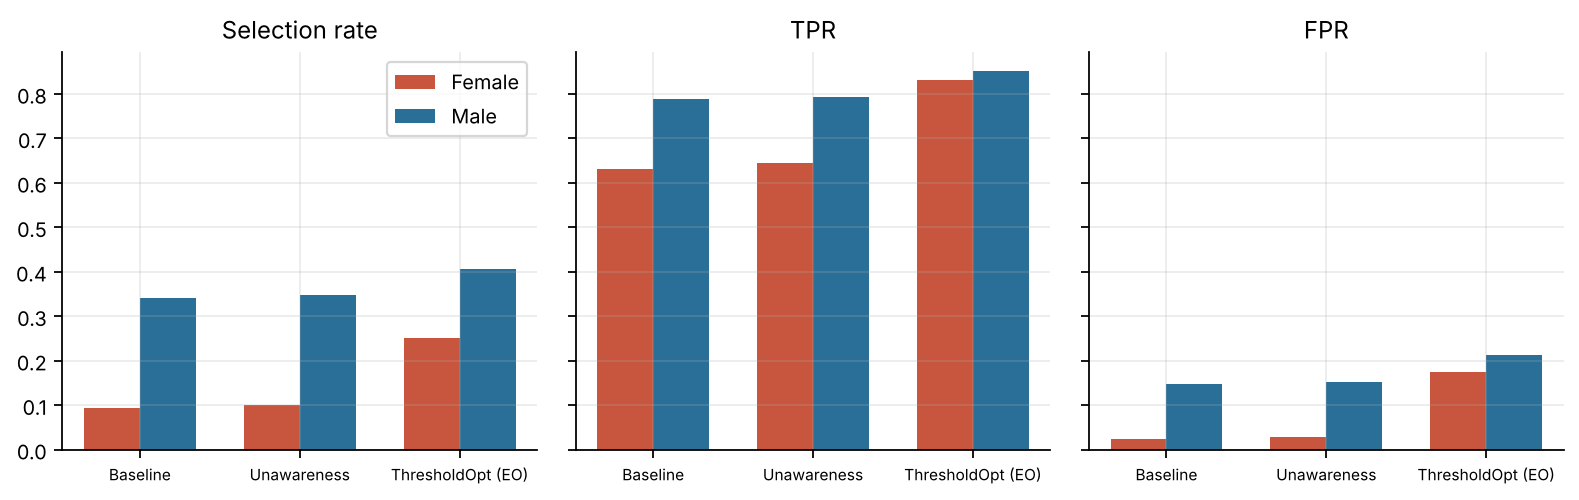
\includegraphics[width=0.92\textwidth]{fairness_groups.png}
\caption{Selection rate, TPR and FPR by sex for the baseline, the ``unawareness'' model and the
equalized-odds post-processing (test set).}
\label{fig:fair}
\end{figure}

\paragraph{Limits.} \code{ThresholdOptimizer} needs \code{sex} at prediction time and applies different
thresholds by group. That is disparate treatment, which may be forbidden in some uses (e.g.\ credit in the
EU or US). In-processing (e.g.\ \code{ExponentiatedGradient}) or pre-processing (reweighing) avoids this at
higher training cost. Its predictions are also randomised near the thresholds, which has to be explained to
users. Finally, a fair classifier on biased historical labels remains a model of a biased world: the audit
should be repeated on recent data.

\section{Serving, tests and reproducibility}
The final pipeline is served by a FastAPI app (\code{src/adult\_poc/api.py}): \code{GET /health} and
\code{POST /predict}, which takes a list of records with the original column names, validates them with
Pydantic (types, ranges, \code{sex} $\in$ \{Male, Female\}, optional missing fields) and returns the raw score,
the isotonic-calibrated probability and the decision at the validation threshold. \code{pytest} covers the
feature transformer, the ECE implementation and the endpoint. Seeds, split sizes and tuning budgets are in
\code{config.yaml}; each step is one script (\code{make all}). The data loader calls \code{fetch\_openml} and
falls back to an identical local copy of the UCI file when OpenML is unreachable (which was the case in our
cloud environment).

\section{Conclusion and critical discussion}
\label{sec:conclusion}
LightGBM inside a single preprocessing Pipeline reaches PR-AUC 0.840 and F1 0.735 on unseen data, a clear
gain over the linear baseline (0.777 / 0.692) and over Random Forest (0.815 / 0.714), with honest
CV-based tuning confirmed by validation and test scores that agree with each other. Main limitations and what
we would change:
\begin{itemize}
  \item \textbf{Imbalance remedy vs calibration.} The ablation shows that threshold moving alone matches class
  weighting on F1 with better-calibrated raw scores. In production we would drop the weights (simpler, one
  less calibration step) or keep the isotonic layer as we do here. Our choice made the calibration problem
  visible, and also fixable.
  \item \textbf{Fairness.} The model reproduces the gender gap of the 1994 data. Post-processing closes the
  equalized-odds gap at a cost of 5 F1 points and worse precision for women. Deploying requires an explicit
  choice of fairness definition, and probably an in-processing method that does not use \code{sex} at
  inference.
  \item \textbf{Data validity.} The census data is from 1994 and \$50K is not inflation-adjusted. The model is a
  proof of concept, not a decision tool for today's population.
  \item \textbf{Statistical uncertainty.} Differences below about 0.01 PR-AUC (2 CV standard deviations) should
  not be over-interpreted; bootstrap confidence intervals on test would be the next step.
\end{itemize}

\section*{Use of AI coding assistants}
We used Claude (Anthropic), an AI assistant, to help write and structure the Python code (pipeline,
tuning, SHAP, calibration, fairness and API scripts) and to draft parts of this report. All
methodological choices, results and interpretations were reviewed, re-run and discussed by the group, and
every member can explain each part.

\section*{Contribution statement}
\begin{center}\small
\begin{tabular}{ll}
\toprule
Member & Main contributions \\
\midrule
Sofyan Hadj-Ali & EDA and split design; feature engineering; repository and README \\
Martin Vallée & Imbalance analysis; model zoo; Optuna tuning and run log \\
Henry Falcon de Longevialle & SHAP explainability; calibration diagnostics \\
Kaled Goatache & Fairness audit and mitigation; FastAPI endpoint and tests \\
All & Report writing, review of all results, oral defense preparation \\
\bottomrule
\end{tabular}
\end{center}

\clearpage
\appendix
\sloppy
\section{Run log: every Optuna trial}
\label{app:runlog}
Source file: \code{artifacts/runs/trials.csv} (also contains run id, timestamp, git commit, std of every
metric and full artifact paths), generated by \code{src/adult\_poc/tuning.py}. All metrics are 5-fold CV means on
the training split; class weights balanced for every trial. Artifacts: ``hist'' $=$
\code{artifacts/plots/optuna\_history\_<model>.png} and \code{artifacts/runs/trials\_<model>\_<run\_id>.json}
(per-trial details); ``model'' $=$ \code{artifacts/runs/best\_params\_<model>.json} and the refitted
\code{artifacts/models/<model>.joblib}. $\star$ marks the selected trial.

{\scriptsize
\setlength{\tabcolsep}{3pt}
\begin{longtable}{llp{5.6cm}ccccccl}
\toprule
Model & Trial & Parameters & PR-AUC & sd & ROC-AUC & F1@0.5 & Brier & s & Artifacts \\
\midrule
\endhead
\inputtable{tables/run_log.tex}
\bottomrule
\end{longtable}}

\end{document}
